\documentclass[11pt]{article}

\usepackage[letterpaper,top=2cm,bottom=2cm,left=2.5cm,right=2.5cm,marginparwidth=1.75cm]{geometry}

%packages
\usepackage{amsmath}
\usepackage{graphicx}
\usepackage{amssymb}
\usepackage{algorithm}
\usepackage{algpseudocode}
\usepackage{color,soul}
\usepackage{mathtools}
% \usepackage{subfig}
\usepackage{subcaption}
\usepackage{caption}

% Edits by John:
% Use hyperref when you're referencing anything - in particular, use the \autoref{} command - it's great. One exception: anything in mathmode should be referenced using \eqref{} instead; \autoref{} calls all mathmode objects "equations", even when they're not equations (definitions, inequalities, propositions, statements, etc.), so it's better to use the \eqref{} function.
\usepackage[colorlinks, linkcolor=blue, citecolor=blue, urlcolor=blue]{hyperref}
% Use the align (or similar) environment, rather than built-in latex commands for math statements. That way, things can be aligned properly and equations will be numbered and referencable. The equation below assigns equation numbers based upon the current section.

\numberwithin{equation}{section}
% Use the amsthm environents to define theorems, remarks, definitions, etc., with commands of the form \begin{definition}[DEFINITION ITTLE]
\usepackage{amsthm}% provides the environments
\theoremstyle{definition}% provides a style for definitions - this affects all downstream \newtheorem statements until \theoremstyle is used again.
\newtheorem{theorem}{Theorem}
\newtheorem{definition}{Definition}[section]% numbers definitions within sections
% The singular of "matrices" is "matrix", not "matrice" - the abnormal singular-plural pair is an importation from Latin.
% Use \url{} for hyperlinks (I changed the pytorch link). I think this is included in hyperref, but it may be in base LaTeX.

\DeclarePairedDelimiter\ceil{\lceil}{\rceil}
\DeclarePairedDelimiter\floor{\lfloor}{\rfloor}
\newcommand{\pluseq}{\mathrel{+}=}
\newcommand{\asteq}{\mathrel{*}=}
\newcommand{\Loss}{L}

\usepackage[dvipsnames]{xcolor}
\usepackage[many]{tcolorbox}

\definecolor{lavender}{RGB}{214, 111, 208}
\colorlet{lavender}{lavender!50}

\newcommand{\hlinfo}[1]{{\sethlcolor{lavender}\hl{#1}}}
\newcommand{\note}[1]{\textcolor{red}{[#1]}}

\usepackage{tikz}

\setlength\parindent{0pt}

\begin{document}

\noindent
\begin{center}
    \section*{\centering{Week 3 Notes}}
    \subsection*{\centering{\emph{Lectures 5 \& 6}}}
    \emph{University of Massachusetts Amherst}, CS389
\end{center}

\section{Multilayer Perceptrons (lecture 5)}

\subsection{Non-linearities}

Examples of non-linearity functions can be refered below

\subsubsection{Sigmoid}

\begin{align}
    \sigma(x) = \frac{1}{1+e^{-x}}
\end{align}

The derivative is:
\begin{align}
    \frac{d}{dx}\sigma(x) = \sigma(x) \cdot (1-\sigma(x))
\end{align}

\subsubsection{Tanh}

\begin{align}
    \text{tanh}(x) = \frac{\text{sinh}(x)}{\text{cosh}(x)} = \frac{e^{x}-e^{-x}}{e^{x}+e^{-x}}
\end{align}

The derivative is:
\begin{align}
    \frac{d}{dx} \text{tanh}(x) = 1 - \text{tanh}^{2}(x)
\end{align}

\subsubsection{ReLU}

\begin{align}
    \text{ReLU}(x) = \text{max}(0, x)
\end{align}

Derivative is:

\begin{align}
    \frac{d}{dx}\text{ReLU}(x) = \begin{cases}
        0 & x < 0 \\
        1 & \text{otherwise}
    \end{cases}
\end{align}

\newpage
\section{Backpropagation (lecture 5)}

% \begin{tcolorbox}[title=Derivation:,colframe=purple,colback=blue!5!white,arc=0pt,fonttitle=\bfseries]
%     The algebraic system define over operator $\star$ , which is \emph{closed} and \emph{associative} is called SEMIGROUP.
% \end{tcolorbox}

% Multiply all partial derivatives along the path from loss to $w_1$

As an example, we can setup a neural network with a single weight in each layer with no bias term like in \autoref{fig:backprop_network}. In each layer, we pass the dot product of the weight and the input through an activation function. The output is then passed onto the next layer in the network as an input. For example, the output of the first layer is $A_1(W_1 X_1)$, which then becomes the input for the second layer. 
\begin{figure}[h]
    \begin{center}
        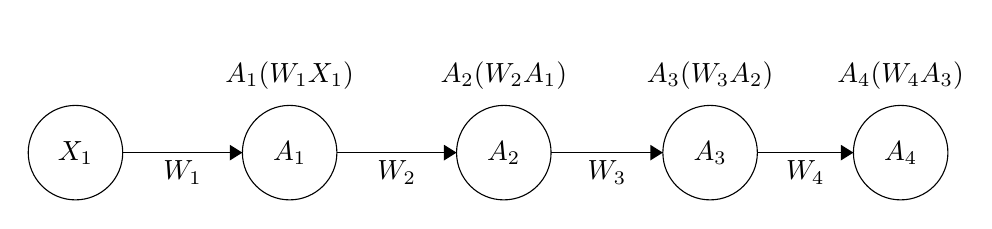
\begin{tikzpicture}[scale=0.2]
        \tikzstyle{every node}+=[inner sep=0pt]
        \draw [black] (16.1,-24.6) circle (3);
        \draw (16.1,-24.6) node {$X_1$};
        \draw [black] (29.7,-24.6) circle (3);
        \draw (29.7,-24.6) node {$A_1$};
        \draw [black] (43.3,-24.6) circle (3);
        \draw (43.3,-24.6) node {$A_2$};
        \draw [transparent] (29.7,-19.7) circle (3);
        \draw (29.7,-19.7) node {$A_1(W_1X_1)$};
        \draw [black] (56.4,-24.6) circle (3);
        \draw (56.4,-24.6) node {$A_3$};
        \draw [transparent] (43.3,-19.7) circle (3);
        \draw (43.3,-19.7) node {$A_2(W_2A_1)$};
        \draw [transparent] (56.4,-19.7) circle (3);
        \draw (56.4,-19.7) node {$A_3(W_3A_2)$};
        \draw [black] (68.5,-24.6) circle (3);
        \draw (68.5,-24.6) node {$A_4$};
        \draw [transparent] (68.5,-19.7) circle (3);
        \draw (68.5,-19.7) node {$A_4(W_4A_3)$};
        \draw [black] (19.1,-24.6) -- (26.7,-24.6);
        \fill [black] (26.7,-24.6) -- (25.9,-24.1) -- (25.9,-25.1);
        \draw (22.9,-25.1) node [below] {$W_1$};
        \draw [black] (32.7,-24.6) -- (40.3,-24.6);
        \fill [black] (40.3,-24.6) -- (39.5,-24.1) -- (39.5,-25.1);
        \draw (36.5,-25.1) node [below] {$W_2$};
        \draw [black] (46.3,-24.6) -- (53.4,-24.6);
        \fill [black] (53.4,-24.6) -- (52.6,-24.1) -- (52.6,-25.1);
        \draw (49.85,-25.1) node [below] {$W_3$};
        \draw [black] (59.4,-24.6) -- (65.5,-24.6);
        \fill [black] (65.5,-24.6) -- (64.7,-24.1) -- (64.7,-25.1);
        \draw (62.45,-25.1) node [below] {$W_4$};
        \end{tikzpicture}
    \end{center}
    \caption{A 4 layer network with a single-weight each layer}
    \label{fig:backprop_network}
\end{figure}

where $A$ is an activation function of any kind. Now recall the equation for the gradient descent update step as well as the gradient of loss:

\begin{align}
    W = W - \alpha \frac{\partial \Loss}{\partial W}
\end{align}

\begin{align}
    \nabla_W \text{Loss} = \frac{\partial \Loss}{\partial W} = \left( \frac{\partial \Loss}{\partial w_1},\, \frac{\partial \Loss}{\partial w_2},\, \ldots,\, \frac{\partial \Loss}{\partial w_m} \right)
\end{align}

Previously, we solved this using the chain rule:
\begin{align}
    \frac{\partial L}{\partial W_j} = \frac{\partial \hat{y}}{\partial w_j} \frac{\partial L}{\partial \hat{y}}
\end{align}

We can extend this chain rule technique and apply it to our network in \autoref{fig:backprop_network}. The idea is to consider all the terms that depend on each other in the network. The reason why we need to do this is because the input of a layer is the output of the previous layer. For example, changing $w_2$ will affect $A_4$, $A_3$, $A_2$ and $L$ so we must consider all these variables when we try to find $\frac{\partial L}{\partial w_2}$. We can do this by multiplying all the partial derivatives along the path from loss to $w_i$:

\begin{align}
    \frac{\partial L}{\partial w_4} = \color{blue} \frac{\partial L}{\partial A_4} \color{black} \cdot \frac{\partial A_4}{\partial w_4}
\end{align}
\begin{align}
    \frac{\partial L}{\partial w_3} = \color{blue} \frac{\partial L}{\partial A_4} \cdot \frac{\partial A_4}{\partial A_3} \color{black} \cdot \frac{\partial A_3}{\partial w_3}
\end{align}
\begin{align}
    \frac{\partial L}{\partial w_2} = \color{blue} \frac{\partial L}{\partial A_4} \cdot \frac{\partial A_4}{\partial A_3} \cdot \frac{\partial A_3}{\partial A_2} \color{black} \cdot \frac{\partial A_2}{\partial w_2}
\end{align}
\begin{align}
    \frac{\partial L}{\partial w_1} = \color{blue} \frac{\partial L}{\partial A_4} \cdot \frac{\partial A_4}{\partial A_3} \cdot \frac{\partial A_3}{\partial A_2} \cdot \frac{\partial A_2}{\partial A_1} \color{black} \cdot \frac{\partial A_1}{\partial w_1}
\end{align}

Observe that a lot of the partial derivattives are repeated, as highlighted in blue. 


%  This calculation doesn't depend on the other gates in the network, and it doesn't require knowledge of the overall structure of the network. Instead, each gate can compute its local gradient independently and pass it along to the gates that feed into it. This makes backpropagation a highly parallelizable and efficient process.

% Notice that backpropagation is a beautifully local process. Every gate in a circuit diagram gets some inputs and can right away compute two things: 1. its output value and 2. the local gradient of its inputs with respect to its output value. Notice that the gates can do this completely independently without being aware of any of the details of the full circuit that they are embedded in


% Vanishing and Exploding gradients


\subsection{Code implementation (lecture 6)}



\begin{thebibliography}{2}
    \bibitem{DrCoop} Cooper.

\end{thebibliography}

\end{document}
